%Este trabalho está licenciado sob a Licença Creative Commons Atribuição-CompartilhaIgual 4.0 Internacional. Para ver uma cópia desta licença, visite https://creativecommons.org/licenses/by-sa/4.0/ ou envie uma carta para Creative Commons, PO Box 1866, Mountain View, CA 94042, USA.

\chapter{Expressões algébricas}

   \vskip0.3cm
 \colorbox{azul}{
 \begin{minipage}{0.9\linewidth}
 \begin{center}
  Expressões algébricas são expressões matemáticas que envolvem números, letras e operações.
 \end{center}
 \end{minipage}}
 \vskip0.3cm

 Como por exemplo:

 \begin{eqnarray*}
  2x=4,\\
  x^2+1=0,\\
  x(x+3)=5,\\
  2x+3y=17,\\
  x^2 + 2y + 3z -4= 52, \\
  \dfrac{14x + 8y}{2x}= 3, \\
  \dfrac{2}{5}x^3 + 3\sqrt{x^4}= 67, \\
  5x(x+3)-4x(2-x)=7.
 \end{eqnarray*}

 Nestas expressões as letras que aparecem são chamadas de \textbf{variáveis}, e os números que aparecem multiplicando uma letra são chamados de \textbf{coeficientes}.

 As expressões algébricas são utilizadas dentre outras coisas, para descrever uma situação problema na qual não conhecemos todos os valores envolvidos, representar uma fórmula, ou expressar uma equação. Devido a sua importância nas exatas precisamos compreender como se comportam as operações presentes nas expressões algébricas, em outras palavras, como fazer contas com letras.

\section{Operações algébricas}

 \vskip0.3cm

 \textbf{Adição e subtração}

 Podemos somar somente letras iguais e com mesmo expoente. Como por exemplo:

 \begin{itemize}
  \item $2x + x= (2+1)x= 3x$;
  \item $x^2 - 3x^2= (1-3)x^2= -2x^2$;
  \item $2x + y + 5x^2 + 7y - 3x= 5x^2 + (2-3)x + (1+7)y= 5x^2 - 1x + 8y$;
  \item $3(x+ 4y-2)= 3x + 3.4y - 3.2= 3x + 12y - 6$;
  \item $\dfrac{3x^2}{4}+\dfrac{x}{2}= \dfrac{3x^2 + 2x}{4}$.
 \end{itemize}

  \vskip0.3cm

 \textbf{Multiplicação}

 Na multiplicação devemos sempre multiplicar coeficiente por coeficiente e letra por letra. Sendo que no caso das letras serem iguais, devemos manter a letra e somar seus expoentes, e no caso das letras serem diferentes apenas fazemos a associação das duas letras. Como mostram os seguintes exemplos:

  \begin{itemize}
   \item $x \cdot x = x^{1+1}= x^2$;
   \item $x \cdot x^2= x^{1+2}= x^3$;
   \item $x \cdot 2y= (1 \cdot 2)xy= 2xy$;
   \item $3x \cdot 2x^2y= (3 \cdot 2)x^{1+2}y= 6x^3y$;
   \item $4x^4 \cdot \dfrac{1}{2x^{2}}= 4x^4 \cdot \dfrac{1}{2}x^{-2}= (4 \cdot \dfrac{1}{2})x^{4-2}= 2x^2$;
   \item $(x - 1) \cdot (x - 2)= x(x-2) - 1(x-2)= x^2 -2x -x +2= x^2 - 3x + 2$.
  \end{itemize}

  \vskip0.3cm

   \textbf{Divisão}

   Na divisão devemos sempre dividir coeficiente por coeficiente e letra por letra. Sendo que no caso das letras serem iguais, devemos manter a letra e subtrair seus expoentes, e no caso das letras serem diferentes apenas fazemos a associação das duas letras. Como mostram os seguintes exemplos:

  \begin{itemize}
   \item $x \div x= x^{1-1}= x^0= 1$;
   \item $x \div x^2= x^{1-2}= x^{-1}= \dfrac{1}{x}$;
   \item $2y \div x= \dfrac{2y}{x}$;
   \item $4y^3 \div 2y^2= \dfrac{4}{2} \cdot \dfrac{y^3}{y^2}= 2y^{3-2}= 2y$;
   \item $\dfrac{x^2yz^3}{x^2y^3z^2}= x^{2-2}y^{1-3}z^{3-2}= x^0 y^{-2}z^{1}= \dfrac{z}{y^2}$;
   \item $\dfrac{(x+3) \cdot (x-1)}{(x-1)\cdot (2x+3)}= \dfrac{x+3}{2x+3}$.
  \end{itemize}

 \vskip0.3cm

  \textbf{Potenciação}

  Na potenciação devemos aplicar o expoente ao coeficiente e à incógnita, obedecendo as propriedades de potência.

    \begin{itemize}
     \item $(2x)^2= 2^2 \cdot x^2= 4x^2$;
     \item $(3x^2)^3= 3^3 \cdot x^{2\cdot 3}= 27x^6$;
     \item $(x+1)^2= (x+1) \cdot (x+1)= x^2 + 2x +1$;
     \item $(x-1)^2= (x-1) \cdot (x-1)= x^2 - 2x +1$;
     \item $\left(\dfrac{3a^2}{4}\right)^2= \dfrac{3^2 a^{2 \cdot 2}}{4^2}= \dfrac{9a^4}{16}$.
    \end{itemize}

  \vskip0.3cm

  \textbf{Radiciação}

  Na radiciação devemos extrair a raiz do coeficiente e da incógnita. Observamos que extrair a raiz da incógnita é equivalente a dividir seu expoente pelo índice da raiz.
    \begin{itemize}
     \item $\sqrt{x}= x^{\frac{1}{2}}$;
     \item $\sqrt{x^2}= \abs{x}$;
     \item $\sqrt{x^4}= (x^4)^{\frac{1}{2}}= x^{\frac{4}{2}}= x^2$;
     \item $\sqrt[3]{8x^6}= \sqrt[3]{8} \cdot \sqrt[3]{x^6}=\sqrt[3]{2^3} \cdot \sqrt[3]{x^6} = 2^{\frac{3}{3}} x^{\frac{6}{3}}= 2x^2$;
     \item $\sqrt{\dfrac{2x^2}{16}}= \dfrac{\sqrt{2x^2}}{\sqrt{4^2}}= \dfrac{\sqrt{2} \cdot \abs{x}}{4}$.
     
    \end{itemize}

 \vskip0.3cm

  \textbf{Fatoração das expressões algébricas}

 \vskip0.3cm

 A fatoração das expressões algébricas, é o que nos permite escrever a expressão como um produto de dois termos, ela é utilizada principalmente na resolução de equações, para acelerar o processo de resolução.

 Os seguintes casos de fatoração são os mais utilizados:
 \begin{itemize}
  \item Fator em comum: $x^2 + x= x(x + 1)$; $4x^2 + 6= 2(2x^2 + 3)$
  \item Agrupamento: $ax + bx + ay + by= (a+b)x+(a+b)y= (a+b)(x+y)$
  \item Trinômio quadrado perfeito (+): 
\begin{equation}
(x + y)^2= (x+y) \cdot (x+y)= x^2 + xy + yx + y^2= x^2 + 2xy + y^2
\end{equation}
  \item Trinômio quadrado perfeito (-): 
\begin{equation}
(x - y)^2= (x - y) \cdot (x - y)= x^2 - xy - yx + y^2 = x^2 - 2xy + y^2
\end{equation}
  \item Diferença de dois quadrados: 
\begin{equation}
(x + y) \cdot (x - y)= x^2 - xy + yx - y^2 = x^2 - y^2
\end{equation}
  \item Cubo perfeito (+): 
\begin{equation}
(x+y)^3= (x+y)^2 \cdot (x+y)= (x^2 + 2xy + y^2) \cdot (x+y)  =x^3 + 3x^2y + 3xy^2 + y^3
\end{equation}
  \item Cubo perfeito (-): 
\begin{equation}
(x-y)^3= (x-y)^2 \cdot (x-y)= (x^2 - 2xy + y^2) \cdot (x-y)= x^3 - 3x^2y + 3xy^2 - y^3
\end{equation}
  \item Diferença de dois cubos:
\begin{equation}
x^3 - y^3= (x-y) \cdot (x^2 + xy + y^2)
\end{equation}
 \end{itemize}
 
 \section{Binômio de Newton}
 
 As expressões $(x + y)^2$ e $(x + y)^3$ para $x, y \in \R$,podem ser generalizadas para $(x + y)^n$ com $n \in \N$, esta generalização é dada pelo Binômio de Newton, da seguinte forma:
 
\begin{equation}
(x + y)^n= \sum^{n}_{k=0} \binom{n}{k} \cdot x^{n-k} y^{k}= \sum^{n}_{k=0} \binom{n}{k} \cdot x^{k} y^{n-k} 
\end{equation}
 
\begin{equation}
(x - y)^n= (x +(-y))^n= \sum^{n}_{k=0} \binom{n}{k} \cdot x^{n-k} (-y)^{k}= \sum^{n}_{k=0} \binom{n}{k} \cdot x^{n-k} (-1)^{k}y^{k}= \sum^{n}_{k=0} (-1)^{k} \binom{n}{k} \cdot x^{n-k} y^{k}
\end{equation}
 
 Os coeficientes $\binom{n}{k}$ são chamados coeficientes binomiais e são definidos por:
 
\begin{equation}
\binom{n}{k}= \frac{n!}{k!(n-k)!}
\end{equation}

 para $n, k \in \N$ com $k \leq n$. 
 
 Vale lembrar que por definição o fatorial de $n$ é dado por:
\begin{equation}
n!= n \cdot (n-1) \cdot (n-2) \cdots 2 \cdot 1 \ .
\end{equation}

 
 \section{Expressões algébricas com frações}
 
 Expressões algébricas com frações:
 \begin{exem}    
  $\dfrac{6x^7 x^6}{3x^3x^8}$
\begin{equation}
\dfrac{6x^7 x^6}{3x^3x^8}= \dfrac{6x^{7+6}}{3x^{3+8}}= \dfrac{6x^{13}}{3x^{11}}= 2x^{13-11}= 2x^2 \ ;
\end{equation}
 \end{exem}
 
 \begin{exem}
  $\dfrac{4x^0y^5z^3}{12z^3y^4x^3}$
\begin{equation}
\dfrac{4x^0y^5z^3}{12z^3y^4x^3}= \dfrac{4x^0y^5z^3}{12x^3y^4z^3}= \dfrac{4}{12} \cdot \dfrac{x^0}{x^3} \cdot \dfrac{y^5}{y^4} \cdot \dfrac{z^3}{z^3}= \dfrac{1}{4} \cdot \dfrac{1}{x^3} \cdot y \cdot 1=\dfrac{y}{3x^3} \ ;
\end{equation}
  \end{exem}
 
 \begin{exem}
  $\dfrac{x^2+2x^5}{x^3}= \dfrac{x^2(1+2x^3)}{x^2 x}= \dfrac{1+2x^3}{x}$;
 \end{exem}
 
 \begin{exem}
  $\left(\dfrac{4x^3y^2}{3z^3}\right) \cdot \left(\dfrac{z}{2x^2y} \right)^3$
\begin{equation}
\left(\dfrac{4x^3y^2}{3z^3}\right) \cdot \left(\dfrac{z}{2x^2y} \right)^3 = \left(\dfrac{4x^3y^2}{3z^3}\right) \cdot \left(\dfrac{z^3}{2^3(x^2)^3y^3} \right)= \dfrac{4x^3y^2z^3}{3z^38x^6y^3}= \dfrac{1}{6x^3y} \ ;
\end{equation}
  \end{exem}
 
 \begin{exem}
 $\dfrac{x^2 - 4}{x^4 - 2x^3}$
\begin{equation}
\dfrac{x^2 - 4}{x^4 - 2x^3}= \dfrac{(x+2) \cdot (x-2)}{x^3 \cdot (x - 2)}= \dfrac{x+2}{x^3} \ ; 
\end{equation}
  \end{exem}
 
 \begin{exem}
  $\dfrac{2y}{z} \cdot \left( \dfrac{z}{x^3} - \dfrac{3z}{x^4y^4} \right) + \left( \dfrac{zy}{x^2} \right)^{-2}$
  
  \begin{eqnarray*}
   \dfrac{2y}{z} \cdot \left( \dfrac{z}{x^3} - \dfrac{3z}{x^4y^4} \right) + \left( \dfrac{zy}{x^2} \right)^{-2} 
   &=& \dfrac{2y}{z} \cdot \left( \dfrac{zxy^4}{x^4y^4} - \dfrac{3z}{x^4y^4} \right) + \left( \dfrac{x^2}{zy} \right)^{2} \\
   &=& \dfrac{2y}{z} \cdot \left( \dfrac{zxy^4 - 3z}{x^4y^4} \right) + \left( \dfrac{x^4}{z^2y^2} \right) \\
   &=& \left( \dfrac{2zxy^5 - 6yz}{x^4y^4z} \right) + \left( \dfrac{x^4}{z^2y^2} \right) \\
   &=& \left( \dfrac{yz(2xy^4 - 6)}{x^4y^4z} \right) + \left( \dfrac{x^4}{z^2y^2} \right) \\
   &=& \left( \dfrac{2xy^4 - 6}{x^4y^3} \right) + \left( \dfrac{x^4}{z^2y^2} \right) \\
   &=& \left( \dfrac{(2xy^4 - 6) \cdot (z^2)}{x^4y^3z^2} \right) + \left( \dfrac{x^4 \cdot (x^4y)}{x^4y^3z^2} \right) \\
   &=& \left( \dfrac{2xy^4z^2 - 6z^2}{x^4y^3z^2} \right) + \left( \dfrac{x^8y}{x^4y^3z^2} \right) \\
   &=& \dfrac{2xy^4z^2 - 6z^2 + x^8y}{x^4y^3z^2} \ ;
  \end{eqnarray*}
 \end{exem}
 
 \begin{exem}
  $\dfrac{2xy-1}{x^2 - y^2} + \dfrac{4x}{x-y}$
  \begin{eqnarray*}
   \dfrac{2xy-1}{x^2 - y^2} + \dfrac{4x}{x-y} &=& \dfrac{2xy-1}{(x-y)\cdot (x+y)} + \dfrac{4x}{x-y} \\
   &=& \dfrac{2xy-1}{(x-y)\cdot (x+y)} + \dfrac{4x \cdot (x+y)}{(x-y)\cdot (x+y)} \\
   &=& \dfrac{2xy - 1 + 4x^2 + 4xy}{(x-y)\cdot (x+y)} \\
   &=& \dfrac{6xy - 1 + 4x^2}{x^2 - y^2} \ ;
  \end{eqnarray*}
  \end{exem}
 
 \begin{exem}
  $\dfrac{-4x^2}{x^3 - y^3} + \dfrac{4}{x-y}$
  \begin{eqnarray*}
   \dfrac{-4x^2}{x^3 - y^3} + \dfrac{4}{x-y} & = & \dfrac{-4x^2}{(x-y)\cdot (x^2+xy+y^2)} + \dfrac{4}{x-y} \\
   &=& \dfrac{-4x^2}{(x-y)\cdot (x^2+xy+y^2)} + \dfrac{4 \cdot (x^2+xy+y^2)}{(x-y)\cdot (x^2+xy+y^2)} \\
   &=& \dfrac{-4x^2 + 4x^2 + 4xy + 4y^2}{(x-y) \cdot (x^2+xy+y^2)} \\
   &=& \dfrac{4xy + 4y^2}{x^3 - y^3}  \ ;
  \end{eqnarray*}
  \end{exem}
 

 
 \section{Expressões algébricas com módulos}
 
 Expressões modulares:

 \begin{exem}
  $\dfrac{\abs{x}}{x}$

  Precisamos analisar separadamente o casos em que $x<0$ e $x>0$, note que o caso em que $x=0$ a expressão não está definida, pois não existe divisão por $0$ (zero), por isso não precisamos nos preocupar com este caso.

  \begin{itemize}
   \item Caso $x> 0$, temos pela definição de módulo que, $\abs{x}= x$, de modo que
\begin{equation}
\dfrac{\abs{x}}{x}=\dfrac{x}{x}= 1
\end{equation}
   \item Caso $x< 0$, temos pela definição de módulo que, $\abs{x}= -x$, de modo que
\begin{equation}
\dfrac{\abs{x}}{x}=\dfrac{-x}{x}= -1
\end{equation}
  \end{itemize}

 Portanto,

  \[ \frac{\abs{x}}{x} = \begin{cases}
      x= -1, \ \ \text{se} \ \ x< 0 \\
      x= 1, \ \ \text{se } \ \ x> 0 \ .
     \end{cases}
  \]
\end{exem}
 
 \begin{exem}
  $\abs{-5x^5}$
\begin{equation}
\abs{-5x^5}= \abs{-5}\cdot \abs{x^5}= 5 \cdot \abs{x^5}
\end{equation}
 Observe que neste caso o expoente de $x$ é um número ímpar, e no item seguinte um número par, por isso temos essa diferença sútil na resposta.
 \end{exem}
 
 \begin{exem}
  $\abs{-5x^4}$
\begin{equation}
\abs{-5x^4}= \abs{-5}\cdot \abs{x^4}= 5 \cdot x^4
\end{equation}
 \end{exem}
 
 \begin{exem}
  $\abs{\dfrac{2x^2y}{4xy^3}}$
\begin{equation}
\abs{\dfrac{2x^2y}{4xy^3}} = \abs{\dfrac{x}{2y^2}}= \dfrac{\abs{x}}{\abs{2y^2}}= \dfrac{\abs{x}}{\abs{2} \cdot \abs{y^2}}= \frac{\abs{x}}{2 \cdot y^2}
\end{equation}
 \end{exem}
 
 \begin{exem}
  $\dfrac{\abs{-6x}}{5} - \abs{\dfrac{-3x}{2}}$

 \begin{eqnarray*}
  \dfrac{\abs{-6x}}{5} - \abs{\dfrac{-3x}{2}} &=&
 \dfrac{\abs{-6}\cdot \abs{x}}{5} - \dfrac{\abs{-3} \cdot \abs{x}}{\abs{2}} \\
 &=& \dfrac{6 \cdot \abs{x}}{5} - \dfrac{ 3 \cdot \abs{x}}{2} \\
 &=& \dfrac{12 \cdot \abs{x}}{10} - \dfrac{15 \cdot \abs{x}}{10} \\
 &=& \dfrac{12\abs{x} - 15\abs{x}}{10} \\
 &=& \dfrac{-3\abs{x}}{10}
 \end{eqnarray*}

\end{exem}

 \begin{exem}
  $\abs{x-2} + \abs{x+4}$ \label{eqmodulo}

 Para simplificar esta expressão, primeiro precisamos usar duas vezes a definição de módulo:

 \[ \abs{x-2} = \begin{cases}
      -(x-2), \ \ \text{se} \ \ (x-2)< 0 \\
      x-2, \ \ \text{se } \ \ (x-2) \geq 0
     \end{cases}
     \Rightarrow
     \abs{x-2} = \begin{cases}
      -x + 2, \ \ \text{se} \ \ x < 2 \\
      x-2, \ \ \text{se } \ \ x \geq 2
     \end{cases}
  \]

 \[ \abs{x+4} = \begin{cases}
      -(x+4), \ \ \text{se} \ \ (x+4)< 0 \\
      x+4, \ \ \text{se } \ \ (x+4) \geq 0
     \end{cases}
     \Rightarrow
     \abs{x+4} = \begin{cases}
      -x - 4, \ \ \text{se} \ \ x < -4 \\
      x + 4, \ \ \text{se } \ \ x \geq -4
     \end{cases}
  \]

  Observe que $\abs{x-2}$ muda de sinal quando $x=2$, e que $\abs{x+4}$ muda de sinal quando $x=-4$, logo esta soma de módulos tem uma definição particular para cada um dos intervalos $(-\infty, -4)$, $[-4, 2)$ e $[2, \infty)$. Para facilitar a compreensão organizamos na tabela abaixo a soma em cada caso.

   \begin{table}[H]
 \centering
 \begin{tabular}{|c|c|c|c|} \hline
 \rowcolor{cinza}
  Expressão & $(-\infty, -4)$ & $[-4, 2)$ & $[2, \infty)$  \\\hline
  $\abs{x-2}$ & $-x+2$ &  $-x+2$ & $x-2$ \\\hline
  $\abs{x+4}$ & $-x-4$ &  $x+4$ & $x+4$ \\\hline
  $\abs{x-2} + \abs{x+4}$ & $-x+2-x-4$ & $-x+2+x+4$ & $x-2+x+4$ \\\hline
 \end{tabular}
\end{table}

 Portanto, temos que

  \[ \abs{x-2} + \abs{x+4} = \begin{cases}
      -2x-2, \ \ \text{se} \ \ x < -4 \\
      6, \ \ \text{se } \ \ -4 \leq x < 2 \\
      2x + 2, \ \ \text{se} \ \ x \geq 2 \ .
     \end{cases}
  \]
 \end{exem}
 
 \newpage
 \section{Expressões algébricas com raízes}
 
 Vejamos alguns exemplos de expressões algébricas com raízes;
 
 \begin{exem}   
   $x^{\frac{5}{7}} \cdot x^{\frac{10}{7}} \cdot x^{\frac{6}{7}}$
\begin{equation}
x^{\frac{5}{7}} \cdot x^{\frac{10}{7}} \cdot x^{\frac{6}{7}}= x^{\frac{5+10+6}{7}}= x^{\frac{21}{7}}= x^3 \ ;
\end{equation}
    \end{exem}
 
 \begin{exem}
   $\dfrac{\sqrt[5]{x^2}}{x} \cdot \dfrac{\sqrt[5]{x^3}}{y^2} \cdot y^{\frac{3}{2}}$
\begin{equation}
\dfrac{\sqrt[5]{x^2}}{x} \cdot \dfrac{\sqrt[5]{x^3}}{y^2} \cdot y^{\frac{3}{2}}= \dfrac{\sqrt[5]{x^{2+3}}}{x} \cdot y^{\frac{3}{2} - 2}= \dfrac{x}{x} \cdot y^{\frac{-1}{2}}= \dfrac{1}{\sqrt{y}}= \dfrac{1}{\sqrt{y}} \cdot \dfrac{\sqrt{y}}{\sqrt{y}}= \dfrac{\sqrt{y}}{y} \ ;
\end{equation}
   \end{exem}
 
 \begin{exem}
    $\sqrt{x^5} \cdot \sqrt[3]{x}$
\begin{equation}
\sqrt{x^5} \cdot \sqrt[3]{x}= x^{\frac{5}{2}} \cdot x^{\frac{1}{3}}= x^{\frac{15+2}{6}} = x^{\frac{17}{6}} = \sqrt[6]{x^{6+6+5}}= \sqrt[6]{x^6 x^6 x^5} =  x^2 \cdot \sqrt[6]{x^5} \ ;
\end{equation}
   \end{exem}
 
 \begin{exem}
   $\sqrt{\sqrt[3]{x^{10}}}$
\begin{equation}
\sqrt{\sqrt[3]{x^{10}}}= (x^{\frac{10}{3}})^{\frac{1}{2}}= x^{\frac{5}{3}}= \sqrt[3]{x^5}= \sqrt[3]{x^3 \cdot x^2}= x \sqrt[3]{x^2} \ ;
\end{equation}
   \end{exem}
 
 \begin{exem}
    $(\sqrt{x} + 2) \cdot (\sqrt{x} - 2)$
\begin{equation}
(\sqrt{x} + 2) \cdot (\sqrt{x} - 2)= (\sqrt{x})^2 - 4= x-4 \ ;
\end{equation}
   \end{exem}
 
 \begin{exem}
  $(\sqrt[3]{x} - 2) \cdot (\sqrt[3]{x^2} + 2 \sqrt[3]{x} + 4)$
\begin{equation}
(\sqrt[3]{x} - 2) \cdot (\sqrt[3]{x^2} + 2 \sqrt[3]{x} + 4)= \sqrt[3]{x^3} + 2\sqrt[3]{x^2} + 4 \sqrt[3]{x} - 2\sqrt[3]{x^2}- 4 \sqrt[3]{x} - 8= x - 8 \ ;
\end{equation}
   \end{exem}
 
 \begin{exem}
  $\dfrac{125^{\frac{1}{3}}}{\sqrt{2x}} \cdot \sqrt{\dfrac{x}{98}}$
\begin{equation}
\dfrac{125^{\frac{1}{3}}}{\sqrt{2x}} \cdot \sqrt{\dfrac{x}{98}}= \sqrt[3]{125} \cdot \sqrt{\dfrac{x}{98 \cdot 2x}}= \sqrt[3]{5^3} \cdot \sqrt{\dfrac{x}{196x}}= 5 \cdot \dfrac{1}{\sqrt{196}}= \dfrac{5}{14} \ ;
\end{equation}
   \end{exem}
 
 \begin{exem}
   $\dfrac{3\sqrt{x}}{x-4} - \dfrac{\sqrt{x}}{\sqrt{x}+2}$
   
   \begin{eqnarray*}
    \dfrac{3\sqrt{x}}{x-4} - \dfrac{\sqrt{x}}{\sqrt{x}+2} &=& \dfrac{3\sqrt{x}}{(\sqrt{x}+2) \cdot (\sqrt{x}-2)} - \dfrac{\sqrt{x}}{\sqrt{x}+2} \\
    &=& \dfrac{3\sqrt{x}}{(\sqrt{x}+2) \cdot (\sqrt{x}-2)} - \dfrac{\sqrt{x} \cdot (\sqrt{x}-2)}{(\sqrt{x}+2) \cdot (\sqrt{x}-2)} \\
    &=& \dfrac{3\sqrt{x} - x + 2\sqrt{x}}{(\sqrt{x}+2) \cdot (\sqrt{x}-2)} \\
    &=& \dfrac{5\sqrt{x} - x}{x-4}
   \end{eqnarray*}

 \end{exem}

 
 \chapter{Polinômios}

  \vskip0.3cm
 \colorbox{azul}{
 \begin{minipage}{0.9\linewidth}
 \begin{center}
  Seja $K= \R \text{ ou } \C$. Um polinômio $p$ na incógnita $x$ e com coeficientes em $K$ (simbolicamente, $p \in K[x]$) é uma expressão da forma
\begin{equation}
p(x)= a_nx^n + a_{n-1}x^{n-1}+ \ldots + a_1x+ a_0= \sum_{i=0}^{n} a_ix^i ,
\end{equation}
  em que os coeficientes $a_n, \ldots, a_0 \in K$, $a_n \neq 0$ e $n \in \N$. O número natural $n$ é chamado de grau do polinômio $p$, e escreve-se $gr(p)= n$. O termo $a_0$ é denominado termo constante de $p$.
 \end{center}
 \end{minipage}}
 \vskip0.3cm

 \begin{obs}
 Os termos polinômio e função polinomial serão considerados como sinônimos e utilizados sem distinção no decorrer deste texto.
 \end{obs}

 Uma função polinomial de grau $0$ é uma função constante; uma função polinomial de grau $1$ é uma função linear (ou, função afim); uma função polinomial de grau $2$ é uma função quadrática.

 Por simplicidade, a partir de agora iremos considerar nossos polinômios sobre $\R$, porém esta teoria pode ser estendida sem muita dificuldade para o corpo dos números complexos.

 \begin{defi}
 Dados um número real $k$ e o polinômio $p(x)= a_nx^n + a_{n-1}x^{n-1}+ \ldots + a_1x+ a_0$, chama-se \emph{valor numérico de $p$ em $k$} ao valor:
\begin{equation}
p(k)= a_nk^n + a_{n-1}k^{n-1}+ \ldots + a_1k+ a_0 \ .
\end{equation}
 \end{defi}

\begin{exem}
Por exemplo, se considerarmos o polinômio $p(x)= x^2 + 7x+10$, temos os seguintes valores numéricos para $p$:
\begin{eqnarray*}
p(-6)&=& (-6)^2 + 7(-6) +10= 4\\
p(-5)&=& (-5)^2 + 7(-5) +10= 0\\
p(-4)&=& (-4)^2 + 7(-4) +10= -2\\
p(-2)&=& (-2)^2 + 7(-2) +10= 0\\
p(0)&=& 0^2 + 7 \cdot 0 +10= 10\\
\end{eqnarray*}
\end{exem}

 \begin{defi}
 Em particular, se $k$ é um número real tal que $p(k)= 0$, dizemos que $k$ é uma \emph{raiz} ou \emph{um zero} de $p$.
 \end{defi}

 \begin{exem}
 Portanto no exemplo anterior temos que $k_1= -5$ e $k_2=-2$ são raízes do polinômio $p(x)= x^2 + 7x+10$.
 \end{exem}

  \begin{defi}
  O polinômio nulo (ou identicamente nulo) é um polinômio da forma $p(x)= 0x^n +0x^{n-1}+ \ldots + 0x+ 0$, ou simplesmente, $p(x)= 0$. Por convenção, o grau deste polinômio será indefinido.
 \end{defi}


  \begin{teo}
  Sejam $p$ e $q$ dois polinômios em $K$, dados por:
\begin{equation}
p(x)= a_nx^n + a_{n-1}x^{n-1}+ \ldots + a_1x+ a_0= \sum_{i=0}^{n} a_ix^i
\end{equation}
\begin{equation}
q(x)= b_nx^n + b_{n-1}x^{n-1}+ \ldots + b_1x+ b_0= \sum_{i=0}^{n} b_ix^i
\end{equation}
  temos que $p=q \Leftrightarrow a_i= b_i$, para todo $i \in \{0, 1, 2, \cdots, n\}$.
 \end{teo}

 \begin{dem}
 Para todo $x \in \R$, temos:
\begin{equation}
a_i= b_i \Leftrightarrow a_i - b_i=0 \Leftrightarrow (a_i - b_i)x^i=0 \Leftrightarrow \sum_{i=0}^{n}(a_i - b_i)x^i= 0 \Leftrightarrow
\end{equation}
\begin{equation}
 \sum_{i=0}^{n}a_i x^i - \sum_{i=0}^{n}b_i x^i = 0 \Leftrightarrow \sum_{i=0}^{n}a_i x^i = \sum_{i=0}^{n}b_i x^i \Leftrightarrow p(x)= q(x)
\end{equation}

 \end{dem}

  Este Teorema mostra que, quando escrevemos um polinômio $p$ na forma
\begin{equation}
p(x)= a_nx^n + a_{n-1}x^{n-1}+ \ldots + a_1x+ a_0
\end{equation}
 com $a_i \in K$, então os números $a_0, \ldots, a_n$ são determinados de modo único.

 Dados dois polinômios
\begin{equation}
p(x)= a_nx^n + a_{n-1}x^{n-1}+ \ldots + a_1x+ a_0= \sum_{i=0}^{n} a_ix^i
\end{equation}
\begin{equation}
q(x)= b_nx^n + b_{n-1}x^{n-1}+ \ldots + b_1x+ b_0= \sum_{i=0}^{n} b_ix^i
\end{equation}
  chama-se \emph{soma} de $p$ com $q$ o polinômio
\begin{equation}
(p+q)(x)= (a_n+ b_n)x^n + (a_{n-1}+b_{n-1})x^{n-1}+ \ldots + (a_1+b_1)x+ (a_0+b_0)= \sum_{i=0}^{n} (a_i+b_i)x^i \ .
\end{equation}

  \begin{teo}
  Se $p$, $q$ e $p+q$ são polinômios não nulos, então o grau do polinômio $p+q$ é menor ou igual ao maior dos números $gr(p)$ e $gr(q)$;
\begin{equation}
gr(p+q) \leq \text{máx}\{gr(p), gr(q)\} \ .
\end{equation}
  \end{teo}

  \begin{teo}
  Se $p$, $q$ e $p \cdot q$ são polinômios não nulos, então o grau do polinômio $p \cdot q$ é igual a soma dos graus de $p$ e $q$;
\begin{equation}
gr(p \cdot q) = gr(p) + gr(q) \ .
\end{equation}
  \end{teo}

  Para funções polinomiais o \emph{Teorema Fundamental da Álgebra} garante a existência de zeros.

  \begin{teo}[Teorema Fundamental da Álgebra]
  Seja $p \in \C[x]$ um polinômio não constante. Então existe um número complexo $z_0$ tal que $p(z_0)=0$.
  \end{teo}

  \begin{dem}
  A demonstração deste resultado pode ser encontrada em livros de Cálculo de uma variável complexa ou Análise Complexa como por exemplo página 119 do (SOARES, 2009).
  \end{dem}

  Como consequência direta do Teorema Fundamental da Álgebra temos o seguinte teorema.

  \begin{teo}
  Todo polinômio de grau $n \geq 1$ possui pelo menos uma raiz real ou complexa.
  \end{teo}

 Observe que estes resultados garantem que todo polinômio possui pelo menos uma raiz complexa, como vamos focar nossos estudos em polinômios sobre $\R$, podemos neste caso ter polinômios que não possuem raízes reais. Ainda sobre as raízes de um polinômio vale destacar o seguinte teorema.

 \begin{teo}
  Seja $p$ um polinômio não nulo em $K$, escrito na forma
\begin{equation}
p(x)= a_nx^n + a_{n-1}x^{n-1}+ \ldots + a_1x+ a_0
\end{equation}
   então $p$ tem no máximo $n$ raízes em $K$.
 \end{teo}

 \begin{teo}
  Sejam $p(x)$, $g(x)$ polinômios sobre o corpo $K$, i.e., polinômios em $K[x]$, e suponhamos que $gr(g) \geq 0$. Então, existem polinômios $q(x)$ e $r(x)$ tais que
\begin{equation}
p(x)= q(x)g(x) + r(x) \ , 
\end{equation}
  em que $gr(r) < gr (g)$. Essas condições permitem determinar os polinômio $q$ e $r$ de modo único.
 \end{teo}

 \begin{dem}
 A demonstração deste teorema pode ser encontrada na página 58 do (LANG, 1972).
 \end{dem}



 \begin{exem}
  Como um exemplo para a divisão de polinômios, façamos a divisão do polinômio $p_1(x)=x^3-4x^2+x+6$ pelo binômio $g_1(x)=x+1$:

 \begin{figure}[H]
 \centering
 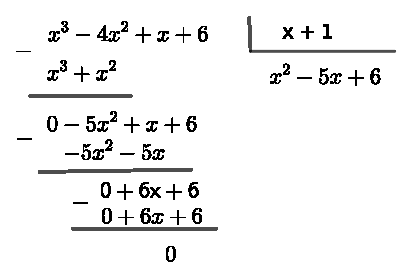
\includegraphics[width=8cm]{./cap_expralg/figs/polinomiosdivisao}
 \end{figure}

 note que o quociente da divisão é $q_1(x)= x^2 - 5x + 6$, e o resto desta divisão é $r(x)=0$ (zero). Como o resto é zero concluímos que $p_1(x)$ é divisível por $g_1(x)$. Portanto $p_1(x)= q_1(x)g_1(x)$, ou seja, $x^3-4x^2+x+6= (x^2-5x+6)(x+1)$.
 \end{exem}

 Como consequência do teorema anterior, temos o seguinte corolário, que nos garante que no exemplo anterior $-1$ é uma raiz do polinômio $p_1(x)$.

 \begin{cor}
 Seja $p$ um polinômio não-nulo sobre $K$. Seja $\alpha \in K$ tal que $p(\alpha)=0$. Então, existe um polinômio $q(x)$ sobre $K$ tal que
\begin{equation}
p(x)= (x - \alpha)q(x) \ .
\end{equation}
 \end{cor}

 Como consequência deste Corolário, todo polinômio de grau $n \geq 1$ pode ser escrito como produto de $n$ fatores de grau $1$.

 \begin{teo}[Teorema da Decomposição]
  Todo polinômio $p(x)= a_nx^n + a_{n-1}x^{n-1}+ \ldots + a_1x+ a_0$, com $a_n \neq 0$, pode ser escrito de forma fatorada
\begin{equation}
p(x)= a_n(x - r_1)(x - r_2) \ldots (x - r_n)
\end{equation}
  onde $r_1, r_2, \cdots, r_n$ são as raízes do polinômio.
 \end{teo}
